\documentclass{article}

\usepackage[T1]{fontenc}
\usepackage{graphicx}
\usepackage{fancyhdr}
\pagestyle{fancy}
\fancyhf{}
\lhead{Version 1.0}
\rhead{Elliot Oram}
\rfoot{\thepage}


\title{Website design}
\author{elo9@aber.ac.uk}

\begin{document}

\maketitle
\tableofcontents

\newpage

\section{Website design diagram}
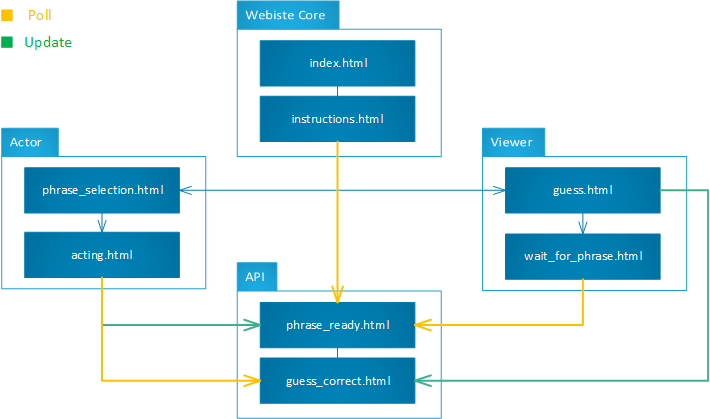
\includegraphics[width=\textwidth]{WebsiteDesign.png}


\section{Description of Website design}
\subsection{Core}
\begin{enumerate}
	\item \textbf{index.html}: The main landing page for the webapp. This will contain an input for the session id that will be used to keep track of the users and will have the option to select either an actor or viewer as the user type.
	
	\item \textbf{instructions.html}: This page will display the instructions on how to play the game. The page contents will differ depending on the user type.
	
	\item \textbf{message\_handler.html}: This class (might be have a different implementation at a later stage) will handle the interaction between the viewers and the actor. The class will send messages between the two main game pages (current\_word.html and guess.html)
	
	\item \textbf{game\_over.html}: This page is displayed once the game concludes and will display the scores of each of the player and a winner. These score may be kept to be used in a leader board.
	
\end{enumerate}


\subsection{Actor}

\begin{enumerate}
	\item \textbf{phrase\_selection.html}: Allows the actor to select the phrase that they wish to act out. The actor will be given the opportunity to guess from a list of five different phrases.
	
	\item \textbf{current\_word.html}: This page will show the current word that the actor is acting and a timer for how long they have remaining. This page will update when a user has guessed the phrase or word correctly. 
	
\end{enumerate}


\subsection{Viewer}

\begin{enumerate}
	\item \textbf{guess.html}: This page will display information about what the actor is acting to the user. The information will include the topic or genre, the current word in the phrase being acted (e.g. word number 3 of 5), the number of letters in that word, and how long until the round ends.
	
\end{enumerate}
 
\end{document}